\documentclass[conference]{IEEEtran}
\usepackage[T1]{fontenc}
\usepackage{amsmath,amssymb}
\usepackage{graphicx}
\usepackage{booktabs}
\usepackage{tabularx}
\usepackage{multirow}
\usepackage{cite}
\usepackage{microtype}
\usepackage{balance}
\usepackage{url}
\usepackage{xcolor}
\usepackage{enumitem}
\usepackage{dblfloatfix}
\graphicspath{{figures/}}
\setlist[itemize]{leftmargin=*,nosep}

\newcommand{\stablecq}{\textsc{StableCQ}}
\newcommand{\tidemark}{\textsc{TideMark}}
\newcommand{\eps}{\varepsilon}

\title{From Input Progress to Answer Stability: Risk-Calibrated Finalization of Streaming Queries}

\author{\IEEEauthorblockN{Adam Kiersztyn\IEEEauthorrefmark{1}, Aneta Oniszczuk\IEEEauthorrefmark{2}, Magdalena Zo{\l}a\IEEEauthorrefmark{3},
Ernest Czerma{\'n}ski\IEEEauthorrefmark{2}, Dariusz Czerwi{\'n}ski\IEEEauthorrefmark{4}}
\IEEEauthorblockA{\IEEEauthorrefmark{1}Department of Computational Intelligence, Lublin University of Technology, Lublin, Poland}
\IEEEauthorblockA{\IEEEauthorrefmark{2}Department of Maritime Transport and Seaborne Trade, University of Gda{\'n}sk, Gda{\'n}sk, Poland}
\IEEEauthorblockA{\IEEEauthorrefmark{3}Department of Computer Science, Lublin University of Technology, Lublin, Poland}
\IEEEauthorblockA{\IEEEauthorrefmark{4}Department of Applied Computer Science, Lublin University of Technology, Lublin, Poland}
\IEEEauthorblockA{Corresponding author: Adam Kiersztyn (a.kiersztyn@pollub.pl)}}

\begin{document}
\maketitle

\begin{abstract}
A record can arrive late without destabilizing its query answer. This distinction is obscured when the decision to finalize a continuous-query result is tied solely to the progress of event time. We study finality as a property of the \emph{answer}, rather than a surrogate for the completeness of its input. The proposed \stablecq{} contract makes that property explicit through a query-dependent loss, an answer tolerance, and an empirical calibration-risk budget. Its operational realization, \tidemark, selects a finalization delay from a small hierarchy of query, time-of-day, and immediately observable activity contexts. The resulting rule is interpretable and leaves watermark-based state retention intact. Evidence comes from a historical replay of 828.9 million maritime records over 4,750 days, evaluated on 44.3 million held-out cell-window-query instances using database processing timestamps as an \emph{audited availability proxy}, not physical network-arrival times. For aligned 15-minute windows, mean finalization delay falls from 60.0 to 18.3 minutes (69.45\%) at 1\% answer tolerance and a 1\% empirical calibration budget; the observed test violation fraction is 0.284\%. A six-configuration sensitivity study reveals the limitation behind that gain: shifting the same nominal window by 5 and 10 minutes reduces the benefit to 36.12\% and 10.66\%, while aligned 60-minute windows yield no latency advantage because the global baseline also finalizes immediately. Empirical violations remain below 1\% in all six settings, without constituting a prospective risk guarantee. The principal contribution is a separation of two operational questions: how far an input has progressed, and when a particular answer carries sufficient evidence to be treated as final.


\end{abstract}

\begin{IEEEkeywords}
stream processing, event time, watermarks, late data, window finalization, query stability, adaptive systems, AIS
\end{IEEEkeywords}

\section{Introduction}
A late record need not destabilize a query \emph{answer}. A vessel message that arrives after a window closes changes its message count, may leave its distinct-vessel count unchanged, and is irrelevant to a speed-filtered query unless it satisfies the predicate. Even when an aggregate changes, the consequence depends on its scale: an increment of one may be material for a count of two but negligible for a count of several thousand. Nevertheless, many stream-processing configurations ultimately tie the declaration of a final answer to an estimate of when further input is unlikely to arrive.

This design choice is understandable, but it conflates two different objects of uncertainty. A watermark expresses progress in the \emph{input-time domain}; the consumer of a continuous query experiences uncertainty in the \emph{answer domain}. The latter depends not only on delay, but on the query operator, the observed answer, and the application's tolerance for revision. The central thesis of this paper is that these two domains should be connected by an explicit, calibratable contract rather than treated as interchangeable.

The distinction builds on a mature body of stream-processing work, from early continuous-query systems \cite{babcock2002streams,abadi2003aurora,golab2003issues,abadi2005borealis,arasu2006cql} to modern event-time semantics and dataflow execution \cite{akidau2015dataflow,fragkoulis2024survey}. Adaptive and keyed watermarks refine how input progress is inferred \cite{awad2019adaptive,yasser2025keyed}; they do not, by themselves, specify how much change in a particular query answer a consumer is willing to accept. The distinction is one of \emph{decision semantics}, not a claim that these mechanisms are defective or should be replaced.

We therefore formulate \stablecq, an answer-finality contract in which the discrepancy between the presently available answer and the closed-corpus answer is measured by a query-specific loss $L_q$. A tolerance $\eps$ describes what the consumer regards as material, and a calibration budget $\alpha$ bounds the \emph{observed frequency} of material discrepancies in a historical calibration period. We then instantiate the contract through \tidemark, a hierarchical policy that selects among candidate delays using the query, hour of day, and activity observed when the window closes. This deliberate economy of context makes it possible to attribute performance gains to answer-aware calibration, rather than to the opacity or capacity of a prediction model.

A consequential part of the investigation is not merely whether the proposed policy works in its nominal setting, but \emph{when its advantage disappears}. Our retrospective corpus contains 828,942,931 typed maritime records over 4,750 contiguous days. The database availability proxy is strongly concentrated at 15-minute boundaries. This makes window phase and duration essential parts of the experimental question. The study accordingly examines six separately calibrated configurations in addition to three query semantics and chronological generalization. In the nominal aligned 15-minute setting, the test population contains 44,282,269 cell-window-query instances; other configurations comprise distinct eligible populations and are therefore compared descriptively, not as paired causal experiments.

Four contributions emerge from this study:
\begin{itemize}
 \item \textbf{A shift in the object of finalization.} We formulate output finality in answer space through a query-dependent loss and an explicit empirical risk budget, without identifying user-visible finality with watermark-based state reclamation.
 \item \textbf{A transparent decision mechanism.} We construct a leakage-safe, hierarchical calibration rule whose context is known at window close. This separates the cost of offline evidence construction from the small online decision table.
 \item \textbf{An auditable large-scale evaluation.} We evaluate three aggregation semantics over a substantial historical corpus, with chronological train/calibration/test separation, day-level robustness analysis, and an audit of the availability timestamp's meaning and cadence.
 \item \textbf{A documented boundary of effectiveness.} Six completed window configurations show that the improvement is substantial but not invariant to window alignment: the same principle can offer a large gain, a modest gain, or no gain when the global rule already finalizes immediately.
\end{itemize}

The result is a qualified but operationally useful claim. \emph{Finality should be determined by what remains uncertain about the answer, provided that the evidence used to quantify that uncertainty is itself audited.} The experiments establish this claim for a specific class of aggregates and a historical availability proxy; they do not establish a distribution-free guarantee or a measured advantage over a live adaptive-watermark implementation.


\begin{figure*}[t]
  \centering
  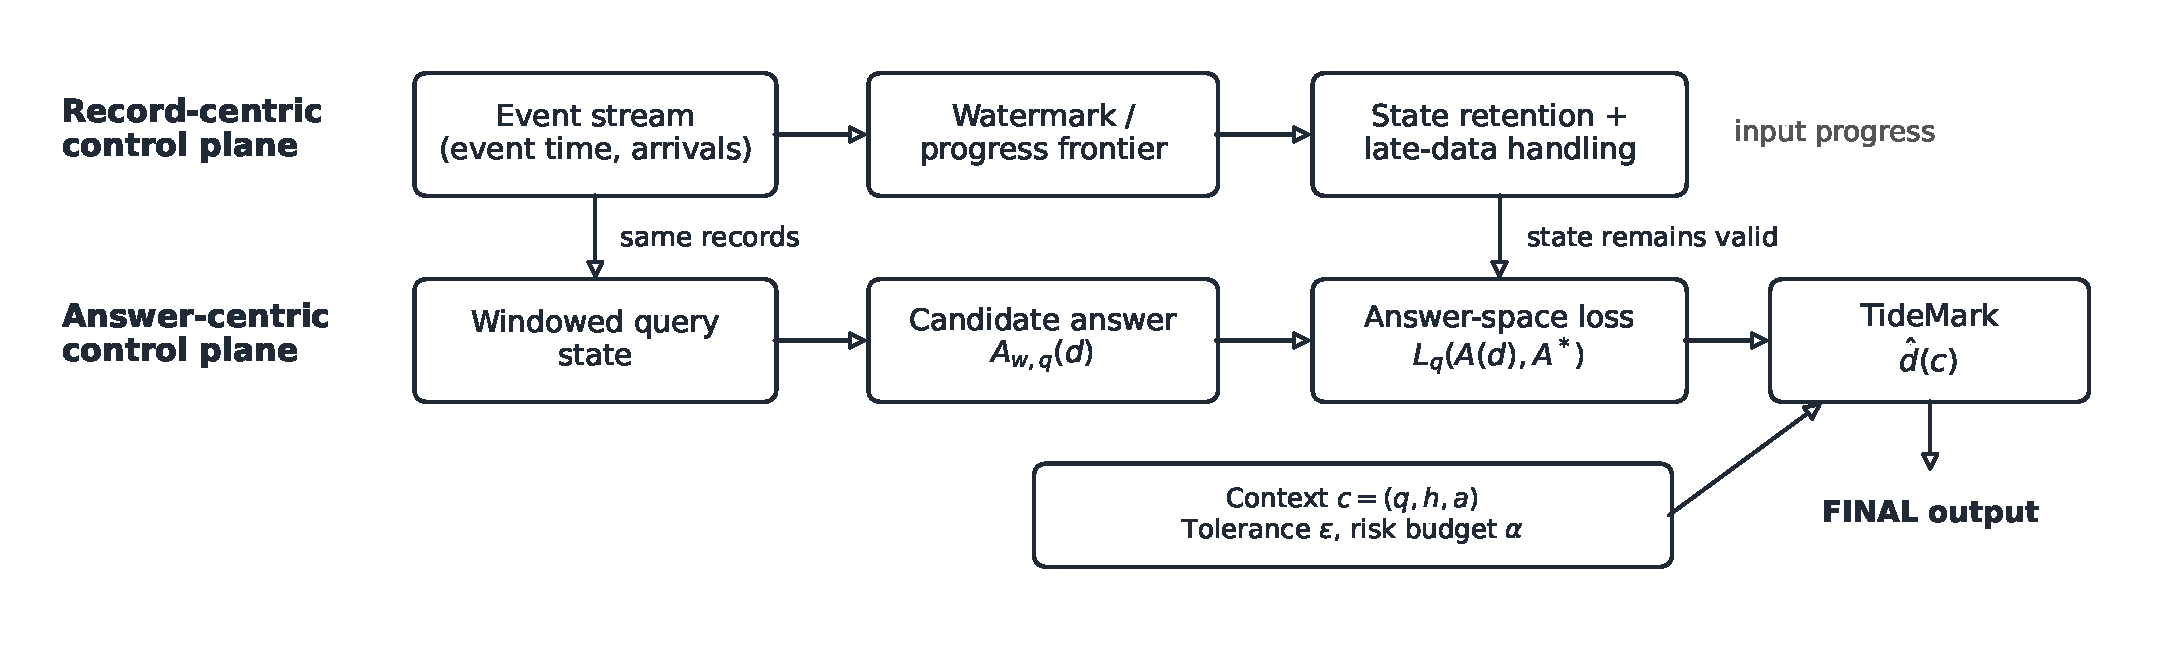
\includegraphics[width=0.98\textwidth]{fig1_stablecq_framework.pdf}
  \caption{Separation of concerns. Record-centric progress remains available for state retention and late-data handling, while \stablecq{} evaluates answer-space loss and \tidemark{} chooses when a query output may be declared final. The two control planes can coexist in the same event-time engine.}
  \label{fig:framework}
\end{figure*}


\section{Related Work}
\subsection{Stream progress, disorder, and window execution}
The first generation of streaming data systems established continuous-query execution as a database problem, in which unbounded input, finite state, and temporal semantics interact \cite{babcock2002streams,abadi2003aurora,golab2003issues,stonebraker2005requirements,abadi2005borealis,arasu2006cql}. Subsequent engines explored different execution abstractions, from micro-batching and timely dataflow to incremental analytics and fault-tolerant state management \cite{zaharia2013dstreams,murray2013naiad,chandramouli2014trill,carbone2017flinkstate}. MillWheel, Flink, and Structured Streaming embody distinct approaches to event-time execution and output generation \cite{akidau2013millwheel,carbone2015flink,armbrust2018structured}; a broader account of their evolution is provided by \cite{fragkoulis2024survey}. These systems make it possible to maintain and revise a windowed result as late records are incorporated, but the conditions under which an application should accept the result as \emph{final} are not necessarily identical to the conditions governing its internal state.

Research on disorder addresses complementary concerns. Out-of-order architectures and adaptive buffering alleviate the computational costs of delayed input \cite{li2008ooo,chandramouli2018impatience}, while specialized aggregation structures, including Scotty, accelerate the processing of windowed results \cite{traub2018scotty,traub2021scotty}. Complex-event processing emphasizes the sensitivity of pattern semantics to arriving records \cite{wu2006cep,cugola2012cep}; transactional approaches provide durability and consistency of state updates \cite{meehan2015sstore}. None of these objectives is equivalent to assessing whether an additional record would change a \emph{particular answer} beyond a specified tolerance.

\subsection{Progress indicators versus answer-level risk}
Watermarks and triggers formalize the relationship between event-time progress and output emission \cite{akidau2015dataflow}. Adaptive watermarks adjust the progress frontier in response to changing arrival behavior \cite{awad2019adaptive}; keyed watermarks make that frontier more granular across heterogeneous substreams \cite{yasser2025keyed}. These are important advances in estimating \emph{input completeness}. Yet the question whether a particular answer will undergo a consequential revision requires a loss function defined on query results. Online aggregation provides an instructive conceptual antecedent for exposing partial answers \cite{hellerstein1997online}, but output-finality decisions based on historical, query-specific revision risk are a distinct operational problem. Our contract therefore supplements, rather than replaces, record-centric progress mechanisms: it calibrates \emph{finalization in answer space} while preserving the engine's existing watermark and state-retention semantics.

\subsection{Maritime data quality and the role of query semantics}
Maritime AIS is a particularly informative domain because apparent timing, record integrity, and downstream interpretation are interconnected but not interchangeable. Earlier studies involving the authors analyzed data integrity, missingness, and anomaly-related issues in AIS repositories \cite{kiersztyn2024aisintegrity} and discussed the dependence of subsequent inference on the quality of AIS records \cite{kiersztyn2025aisaccuracy}. Other published AIS studies by the authors considered operational patterns in offshore passenger-vessel activity \cite{czerwinski2023offshore} and temporal-spatial features for predicting vessel movement status \cite{kiersztyn2025vesselstatus}. These contributions support the choice of AIS as a rich, heterogeneous evaluation domain; they neither propose an answer-finality contract nor report the experiments evaluated here. In particular, \emph{anomalous or imperfect maritime observations should not be equated with late arrival or answer instability}. The present work instead asks, for each query and each audited availability context, when further input is likely to change the answer materially.

\section{Decision Semantics and Design Motivation}
\subsection{Two distinct operational decisions}
Event-time processing serves two purposes that can be coordinated without being identified. A \emph{progress frontier} helps the engine manage out-of-order input, internal state, and the timing of provisional results. An \emph{answer-finality decision}, in contrast, asks whether the residual uncertainty in an exposed query answer is small enough for a given consumer. Progress estimates can help schedule or constrain that decision, but they do not encode the consumer's loss function. Conversely, a decision to accept an approximate answer does not justify discarding the underlying state that may still be needed for corrections or other queries.

\subsection{Why input completeness and answer stability differ}
Consider a 15-minute window with three queries: total message count, number of distinct vessels, and number of vessels whose speed exceeds a threshold. A late record necessarily changes the first query, but may leave the second unchanged if its vessel was already observed and may leave the third unchanged if it fails the speed predicate. Even for the message count, a change from 1 to 2 is qualitatively different from a change from 1,001 to 1,002 if an application tolerates relative error.

This exposes a useful separation between a \emph{progress frontier}, which summarizes what the engine knows about event-time completeness, and an \emph{answer-decision frontier}, which marks the earliest empirically acceptable finalization of a specified query output. Their order need not coincide: an answer can be stable before the input is complete, and a watermark cannot by itself certify that a user's loss tolerance is met. The claim is intentionally restricted to the answer semantics and the reference population used for calibration; it does not confer permission to reclaim state prematurely.

Table~\ref{tab:positioning} makes the distinction precise. Fixed, adaptive, and keyed watermarks differ in how finely they estimate input progress; Dataflow-style triggers provide flexible emission timing. None of these mechanisms, by itself, defines finality through an application-level loss between the current and eventual \emph{query answer}. \stablecq{} introduces that missing decision object and can therefore coexist with any of them.

\begin{table*}[t]
\caption{Positioning of event-time progress and output-finalization mechanisms. ``Answer loss'' means that the finalization decision is explicitly parameterized by the change of a query result, rather than by record lateness alone.}
\label{tab:positioning}
\centering
\small
\resizebox{\textwidth}{!}{%
\begin{tabular}{llllll}
\toprule
Mechanism & Primary decision object & Granularity & Query semantics & Answer tolerance & Main role \\
\midrule
Fixed watermark & Event-time frontier & Stream / partition & No & No & Progress, state cleanup \\
Adaptive watermark \cite{awad2019adaptive} & Learned arrival progress & Stream & No & No & Adaptive progress \\
Keyed watermark \cite{yasser2025keyed} & Event-time frontier & Key / substream & Key identity & No & Fine-grained progress \\
Dataflow triggers \cite{akidau2015dataflow} & Pane emission condition & Window / trigger & User-defined & Not intrinsic & Early/on-time/late output \\
\stablecq{} + \tidemark{} & Query-answer loss/risk & Query + context & Yes & Yes & User-visible finality \\
\bottomrule
\end{tabular}}
\end{table*}

\section{An Explicit Contract for Answer Finality}
Let $w$ be an event-time window and $q$ a query. Let $A_{w,q}^{\star}$ denote the answer obtained after replaying all eligible records assigned to $w$ in the closed corpus. For a candidate finalization delay $d\geq 0$, measured from the end of the event-time window, let $A_{w,q}(d)$ be the answer using only records whose reconstructed availability time is no later than the window end plus $d$.

\stablecq{} is parameterized by a nonnegative query-specific loss
\begin{equation}
 e_{w,q}(d)=L_q\!\left(A_{w,q}(d),A_{w,q}^{\star}\right),
 \label{eq:error}
\end{equation}
so different output types can express different notions of material change. For the count queries evaluated here, all materialized windows have $A_{w,q}^{\star}>0$ and we instantiate
\begin{equation}
 L_q(a,b)=\frac{|b-a|}{b}.
 \label{eq:relerr}
\end{equation}
Given an application tolerance $\eps\geq 0$, a window violates the stability contract at delay $d$ when
\begin{equation}
 V_{w,q}(d;\eps)=\mathbb{I}[e_{w,q}(d)>\eps].
 \label{eq:violation}
\end{equation}
For a context $c$, the population quantity of interest is the conditional violation risk
\begin{equation}
 R_c(d;\eps)=\Pr(V_{w,q}(d;\eps)=1\mid c).
 \label{eq:risk}
\end{equation}
In a historical calibration set, we estimate this quantity by the empirical fraction $\widehat R_c(d;\eps)$. The \stablecq{} decision rule is then to choose the earliest candidate delay whose empirical risk is within a user-selected budget $\alpha$:
\begin{equation}
 \widehat d(c)=\min\{d\in D:\widehat R_c(d;\eps)\leq \alpha\}.
 \label{eq:rule}
\end{equation}
If no candidate satisfies the condition, the largest candidate is selected. We call $\alpha$ an \emph{empirical calibration risk budget}. Equation~\eqref{eq:rule} is not presented as a distribution-free probabilistic guarantee; temporal distribution shift can make test risk differ from calibration risk. This distinction is important in our results.

The contract governs \emph{output finality}, not safe state reclamation. A runtime may declare a result final under \stablecq{} while retaining the underlying event-time state according to its ordinary watermark or retention policy. If a post-final record changes the answer beyond the accepted semantics, the application may log it, issue a correction/retraction, or deliberately ignore it. Thus \stablecq{} does not weaken the engine's record-level correctness machinery; it adds an explicit approximate-finality interface for consumers willing to trade bounded answer risk for latency.

The candidate set used in the experiment spans immediate finalization through 24 hours:
\begin{align*}
D=\{&0,30,60,120,300,600,900,1200,1800,\\
&3600,7200,14400,28800,86400\}\;\text{s}.
\end{align*}
The dense early grid captures low-latency decisions, while longer candidates protect against heavy-tailed historical availability delays.

\section{Hierarchical Calibration of Finalization Decisions}
\subsection{Leakage-safe context construction}
\tidemark{} conditions finalization on $c=(q,h,a)$, where $q$ is the query, $h\in\{0,\ldots,23\}$ is hour of day, and $a$ is an activity bin. Activity is derived from the immediate answer $A_w(0)$, because this quantity is available when the window closes. Query-specific bin boundaries are learned on the training period only and frozen before calibration and testing. Four activity bins are targeted; ties and sparse support can yield fewer effective bins for a query.

For the full run, the train-derived cut points for message count are 0, 2, and 8; for distinct vessels they are 0, 1, and 4; for high-speed vessels the effective cut points are 1 and 2. This construction is intentionally coarse. It captures the intuition that low-count windows are more sensitive to one late item while keeping the policy interpretable.

\subsection{Hierarchical calibration and fallback}
A fine-grained context is only used when at least 200 calibration windows support it. Otherwise the policy backs off through
\begin{equation}
(q,h,a)\rightarrow(q,a)\rightarrow q\rightarrow \text{global}.
\end{equation}
At each level, \tidemark{} applies Eq.~\eqref{eq:rule}. This hierarchy avoids unstable rules for sparse contexts while preserving specialization where evidence is abundant. The resulting model is a compact lookup table, not a learned black box.

\subsection{Baselines and oracle}
We compare \tidemark{} with three references. \emph{Fixed-global} learns one delay for all queries and contexts and is the closest controlled analogue of a single lateness allowance. \emph{Query-static} learns one delay per query, retaining query sensitivity but ignoring hour and activity. \emph{Offline oracle} selects, for each test window, the smallest candidate delay that actually meets the tolerance when compared with $A_{w,q}^{\star}$. It uses future information and is therefore an unattainable lower bound, not an online baseline. We do not present Adaptive or Keyed Watermarks as empirical baselines because they optimize input-progress estimation inside a live engine and require online arrival semantics that this retrospective corpus does not provide; Table~\ref{tab:positioning} therefore treats them as complementary mechanisms rather than as interchangeable policies.

\subsection{Materialization and execution}
The replay materializes candidate answers in a wide representation: each nonempty cell-window-query row stores $A_{w,q}(d)$ for all candidate delays. The latest pipeline partitions output by split, query, and calendar month, uses Zstandard-compressed Parquet, and constructs snapshots in resumable chunks with automatic bisection if memory pressure occurs. Calibration and evaluation then operate on these materializations. This design separates the expensive closed-corpus replay from policy evaluation, allowing many $(\eps,\alpha)$ settings to be tested without rebuilding snapshots.

\subsection{Runtime integration and control-path cost}
In a live engine, \tidemark{} sits on the output-control path rather than the per-record data path. When a window closes in event time, the query operator exposes the immediate provisional answer $A_{w,q}(0)$ and the context features needed by the controller. A constant-time lookup returns $\widehat d(c)$. The operator continues to process late records according to the engine's existing event-time semantics and emits a \emph{final} marker for the answer at window-end plus $\widehat d(c)$. Watermarks may independently retain or evict state. Consequently, \stablecq{} can be introduced without redefining the engine's event-time frontier.

For each $(\eps,\alpha)$ pair, the current experiment stores only 279 calibrated rules across all hierarchy levels. Online inference therefore requires neither a model server nor per-record prediction. Offline calibration evaluates $|D|$ candidate delays over the supported contexts; the expensive operation is building closed-corpus answer snapshots, not applying the policy. This division is important for the systems interpretation: the proposed mechanism changes \emph{when output becomes final} and has a small rule-table representation; full runtime overhead requires direct measurement.

\section{Experimental Setting and Timestamp Semantics}
\subsection{Historical AIS corpus}
The source file contains 154.86 GB of semicolon-delimited AIS-derived records. After typed ingestion, 828,942,931 rows remain in the corpus. Event time spans from 31 December 2011 to 31 December 2024, with 4,750 contiguous calendar days selected for experiments. The approximate number of distinct MMSI identifiers is 297,671. Table~\ref{tab:protocol} summarizes the main protocol.

\begin{table}[t]
\caption{Full-run protocol.}
\label{tab:protocol}
\centering
\resizebox{\columnwidth}{!}{%
\begin{tabular}{ll}
\toprule
Property & Setting \\
\midrule
Typed records & 828,942,931 \\
Contiguous days & 4,750 \\
Train / calibration / test & 2,850 / 950 / 950 days \\
Test interval & 27 May 2022--31 Dec. 2024 \\
Window size & 15 min \\
Spatial cell & $0.25^{\circ}\times0.25^{\circ}$ \\
Queries & messages, distinct vessels, high-speed vessels \\
Speed predicate & $\geq12$ kn; valid speed $\leq70$ kn \\
Activity bins & 4 (train-derived, query-specific) \\
Minimum context support & 200 windows \\
Tolerance $\eps$ & 0, 0.01, 0.05 \\
Risk budget $\alpha$ & 0.01, 0.05 \\
Bootstrap & 1,000 replicas by day \\
\bottomrule
\end{tabular}}
\end{table}

The split is strictly chronological: 2,850 days for training, 950 for calibration, and the final 950 for testing. Activity thresholds are estimated on train only; delay rules are fit on calibration only; all reported policy comparisons use the held-out test period. The materialized evaluation population consists of eligible, nonempty cell-window-query instances with positive closed-corpus answers; we do not claim performance on the potentially much larger population of empty spatial windows.

\subsection{Availability semantics and audit}
The source provides \texttt{MovementDateTime}, used as event time, and \texttt{ProcessedDate}, used to reconstruct when a record became available to the historical database. We emphasize that \texttt{ProcessedDate} is \emph{not verified network reception time}. Consequently, our evaluation is a closed-corpus reconstruction of historical availability, not a claim about live AIS packet transport.

For each record, the raw proxy delay is \texttt{ProcessedDate} minus event time. Across the full typed corpus, the median is 88.5 s, the 90th percentile 643.4 s, the 95th percentile 1,246.4 s, and the 99th percentile 3,361.5 s. On our discrete candidate grid, a record-centric policy designed around the 99th percentile would therefore wait 60 minutes, matching the conservative delay selected by the strict fixed-global baseline. For snapshot construction we use arrival delay relative to the \emph{window end}, clipped at zero: records already available before the end of their window contribute at $d=0$.

A separate cadence audit scans 827,715,328 eligible rows. It finds that 96.870746\% of \texttt{ProcessedDate} values occur at phase zero modulo 900 s. An independent recomputation of all three query snapshots for a held-out day (14 September 2023) matches the materialized snapshots exactly. Figure~\ref{fig:cadence} shows the resulting availability bands and phase structure. These checks support the conclusion that the plateaus seen in answer curves are induced by the recorded availability timestamps rather than a snapshot bug, while preserving the caveat that these timestamps reflect source/database semantics rather than physical packet arrival.

\begin{figure*}[t]
  \centering
  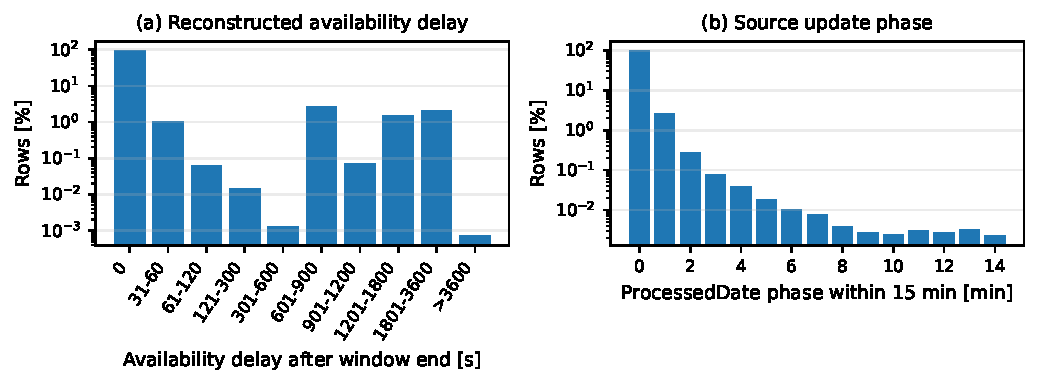
\includegraphics[width=0.95\textwidth]{fig2_availability_cadence.pdf}
  \caption{Availability-proxy audit. (a) Distribution of record availability delay relative to window end. (b) Phase of \texttt{ProcessedDate} within 15-minute intervals. The strong phase concentration motivates explicit source-semantic auditing before interpreting replay latency as network latency.}
  \label{fig:cadence}
\end{figure*}

\subsection{Queries and metrics}
We evaluate three cell-level 15-minute aggregate queries: (i) message count, (ii) number of distinct MMSI values, and (iii) number of distinct vessels with speed at least 12 knots. The first reacts to every eligible late record, the second only to late records introducing a previously unseen vessel, and the third adds predicate selectivity.

The test split contains 20,274,085 message-count windows, 20,274,085 distinct-vessel windows, and 3,734,099 high-speed windows, for 44,282,269 cell-window-query instances in total. We report mean, median, and 95th-percentile finalization delay, violation fraction from Eq.~\eqref{eq:violation}, and mean relative error. Confidence intervals are estimated through 1,000 bootstrap resamples over test days; we use the raw aggregate values in the main tables because they directly weight every evaluated window.

\section{Experimental Evidence}
\subsection{RQ1: How quickly do answers stabilize?}
Figure~\ref{fig:curves} plots the empirical held-out error and $\eps=0.01$ violation curves up to one hour. The message-count and distinct-vessel queries exhibit pronounced steps around 15, 30, and 60 minutes, consistent with the audited source cadence. High-speed-vessel answers are substantially less sensitive in aggregate because fewer records satisfy the predicate. The figure also demonstrates why a single lateness threshold is inefficient: queries share the same input availability process but have different answer responses.

\begin{figure*}[t]
  \centering
  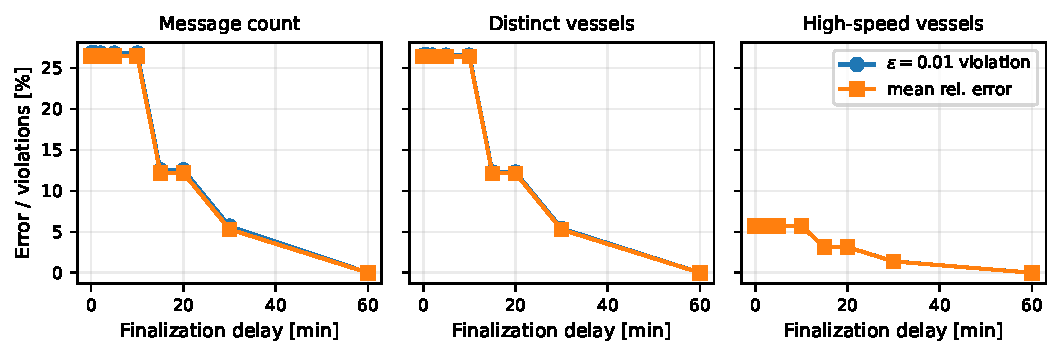
\includegraphics[width=0.98\textwidth]{fig3_delay_quality_curves.pdf}
  \caption{Held-out answer quality versus finalization delay. Curves are query-dependent even though all queries observe the same reconstructed availability process. Values shown through 60 minutes; the experiment evaluates candidates up to 24 hours.}
  \label{fig:curves}
\end{figure*}

\subsection{RQ2: Does context-aware finalization reduce latency?}
Table~\ref{tab:policies} reports the main results for $\eps=0.01$. Under the stricter calibration budget $\alpha=0.01$, both static policies select 60 minutes. Their held-out violation fraction is only 0.0156\%, showing that a single calibrated threshold is strongly conservative. \tidemark{} lowers the mean delay to 18.33 minutes, with median delay 0 and 95th percentile 60 minutes. This is a 69.45\% reduction in mean latency while the observed violation fraction remains 0.284\%, well below 1\%.

At $\alpha=0.05$, fixed-global selects 30 minutes and reaches a 5.202\% held-out violation fraction, slightly exceeding the calibration budget under temporal shift. Query-static remains conservative at 56.21 minutes and 0.280\% violations. \tidemark{} reaches 16.30 minutes and 0.414\% violations. Relative to query-static, the mean-delay reduction is 71.0\%. The offline oracle requires 7.11 minutes on average, indicating that substantial headroom remains for richer context or online adaptation.

\begin{table*}[t]
\caption{Policy comparison on the 44.3M-instance test split for $\eps=0.01$. Violation and mean error are percentages. The oracle uses the closed-corpus answer and is only a lower bound.}
\label{tab:policies}
\centering
\begin{tabular}{llrrrrr}
\toprule
$\alpha$ & Policy & Mean delay [min] & Median [s] & P95 [s] & Violation [\%] & Mean error [\%] \\
\midrule
0.01 & Fixed-global & 60.00 & 3600 & 3600 & 0.0156 & 0.0093 \\
0.01 & Query-static & 60.00 & 3600 & 3600 & 0.0156 & 0.0093 \\
0.01 & \tidemark{} & \textbf{18.33} & \textbf{0} & 3600 & 0.2844 & 0.0433 \\
0.01 & Offline oracle & 7.11 & 0 & 3600 & 0.0003 & 0.0004 \\
\midrule
0.05 & Fixed-global & 30.00 & 1800 & 1800 & 5.2024 & 4.9619 \\
0.05 & Query-static & 56.21 & 3600 & 3600 & 0.2799 & 0.2733 \\
0.05 & \tidemark{} & \textbf{16.30} & \textbf{0} & 3600 & 0.4135 & 0.1722 \\
0.05 & Offline oracle & 7.11 & 0 & 3600 & 0.0003 & 0.0004 \\
\bottomrule
\end{tabular}
\end{table*}

Figure~\ref{fig:tradeoff} visualizes this trade-off. The fixed-global policy can buy latency by accepting substantial test risk, while query-static avoids that risk at the cost of long waits. \tidemark{} occupies a more favorable region because it spends waiting time where the answer is fragile and finalizes immediately where historical evidence supports stability.

\begin{figure}[t]
  \centering
  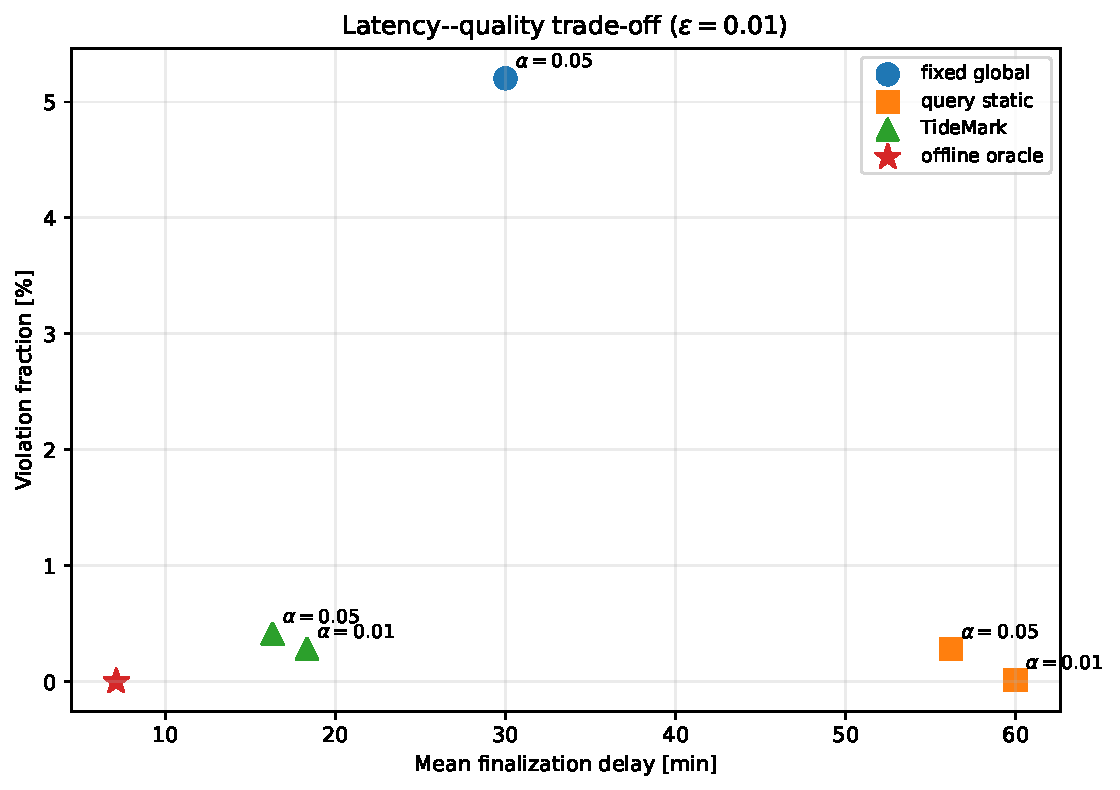
\includegraphics[width=\columnwidth]{fig4_policy_tradeoff.pdf}
  \caption{Mean finalization delay versus observed test violation fraction at $\eps=0.01$. The two points per online policy correspond to $\alpha\in\{0.01,0.05\}$.}
  \label{fig:tradeoff}
\end{figure}

\subsection{RQ3: Which queries benefit from adaptation?}
The query-level decomposition in Table~\ref{tab:query} explains the aggregate result. At $\alpha=0.01$, query-static uses 60 minutes for every query. \tidemark{} reduces mean delay for message count and distinct vessels to 15.83 minutes, whereas high-speed vessels still require 45.45 minutes on average under the learned contexts. Despite this longer selected delay, the high-speed query has the lowest observed violation rate (0.0044\%), because predicate selectivity makes many late records irrelevant to the answer.

\begin{table}[t]
\caption{Query-level results, $\eps=0.01$, $\alpha=0.01$.}
\label{tab:query}
\centering
\resizebox{\columnwidth}{!}{%
\begin{tabular}{llrr}
\toprule
Policy & Query & Mean delay [min] & Viol. [\%] \\
\midrule
Query-static & Message count & 60.00 & 0.0188 \\
Query-static & Distinct vessels & 60.00 & 0.0148 \\
Query-static & High-speed vessels & 60.00 & 0.0025 \\
\midrule
\tidemark{} & Message count & 15.83 & 0.4408 \\
\tidemark{} & Distinct vessels & 15.83 & 0.1796 \\
\tidemark{} & High-speed vessels & 45.45 & 0.0044 \\
\midrule
Oracle & Message count & 7.69 & 0.0004 \\
Oracle & Distinct vessels & 7.52 & 0.0003 \\
Oracle & High-speed vessels & 1.76 & 0.0001 \\
\bottomrule
\end{tabular}}
\end{table}

The learned rules make the role of activity especially clear. Figure~\ref{fig:rules} shows the most-specific rules for $\alpha=0.05$. For message and distinct counts, the lowest-activity quartile usually receives a 60-minute delay, whereas higher-activity windows can often be finalized at the window boundary. The high-speed query exhibits intermediate 15--30 minute decisions in its sparsest supported contexts. Hour-of-day contributes less structure than activity in this corpus, suggesting that activity is the dominant lightweight explanatory feature.

\begin{figure*}[t]
  \centering
  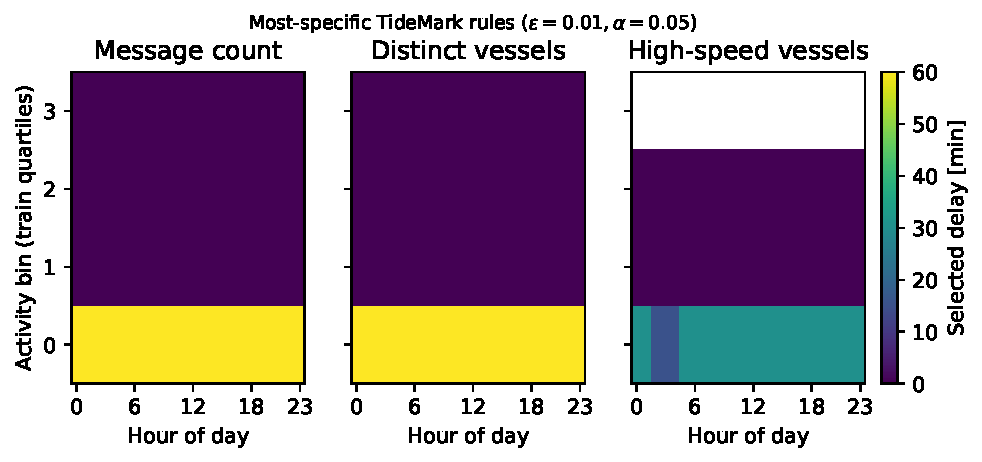
\includegraphics[width=0.92\textwidth]{fig5_context_rules.pdf}
  \caption{Most-specific \tidemark{} rules for $\eps=0.01$, $\alpha=0.05$. White cells have no supported most-specific context and use a fallback level. Activity is defined from training-only quartiles of the immediate answer.}
  \label{fig:rules}
\end{figure*}

\subsection{RQ4: How robust is the calibration under time?}
The held-out test interval is the latest 950 days, rather than an i.i.d. random split. This design intentionally exposes temporal shift. The fixed-global $\alpha=0.05$ rule is an instructive case: its calibration choice of 30 minutes produces 5.20\% aggregate test violations, slightly above the nominal budget. In contrast, the finer \tidemark{} contexts remain substantially below the same budget at 0.414\%. The result should not be read as a formal guarantee; rather, it shows that query- and activity-specific calibration is less brittle than a single global cutoff on this replay.

Table~\ref{tab:daily} adds a day-level view. For $\alpha=0.01$, \tidemark{} exceeds a 1\% daily violation fraction on only 2 of 950 held-out days; its 95th percentile daily violation fraction is 0.484\%. At $\alpha=0.05$, no \tidemark{} test day exceeds 5\%, whereas the fixed-global 30-minute rule exceeds the nominal budget on 460 days. Query-static is also temporally conservative but pays substantially higher latency (Table~\ref{tab:policies}). These daily summaries weight each day equally and therefore complement, rather than replace, the raw instance-weighted metrics.

\begin{table}[t]
\caption{Temporal robustness across 950 held-out days, $\eps=0.01$. Values are computed from daily policy summaries.}
\label{tab:daily}
\centering
\resizebox{\columnwidth}{!}{%
\begin{tabular}{llrrr}
\toprule
$\alpha$ & Policy & Mean daily viol. [\%] & P95 daily [\%] & Days $>\alpha$ \\
\midrule
0.01 & Fixed-global & 0.0145 & 0.0429 & 2 / 950 \\
0.01 & Query-static & 0.0145 & 0.0429 & 2 / 950 \\
0.01 & \tidemark{} & 0.2665 & 0.4844 & 2 / 950 \\
\midrule
0.05 & Fixed-global & 4.9697 & 7.4365 & 460 / 950 \\
0.05 & Query-static & 0.2842 & 0.4179 & 0 / 950 \\
0.05 & \tidemark{} & 0.3990 & 0.6233 & 0 / 950 \\
\bottomrule
\end{tabular}}
\end{table}

Day-bootstrap analysis over 1,000 replicas supports the stability of the qualitative ranking. For $\eps=0.01$, $\alpha=0.01$, the day-macro bootstrap mean delay for \tidemark{} is approximately 17.9 minutes with a 95\% interval of 17.7--18.1 minutes, compared with exactly 60 minutes for the static policies. Differences between day-macro bootstrap estimates and the raw aggregate metrics arise from weighting days equally rather than weighting every cell-window instance equally.

\subsection{RQ5: Does adaptation persist in harder held-out regimes?}
The aggregate test metric could conceal a policy that works only on easy days. We therefore stratify the 950 held-out days twice, using quartiles of the observed daily 95th-percentile source delay and quartiles of daily eligible record volume. These quantities are used only for retrospective stress analysis; they do not enter the learned policy. Table~\ref{tab:stress} reports the day-macro behavior of \tidemark{} at $\eps=0.01$, $\alpha=0.01$. As the source-delay regime becomes harder, the policy increases its mean finalization delay from 14.12 to 21.34 minutes. Mean violation fraction also rises, but remains 0.416\% even in the highest-lateness quartile, and the 95th percentile of daily violation remains below 0.60\%. The activity stratification shows the same qualitative response, with delay increasing from 15.08 to 21.34 minutes as daily volume moves from the lowest to highest quartile. The corresponding fixed-global and query-static policies remain at 60 minutes in every slice.

\begin{table}[t]
\caption{Held-out stress slices for \tidemark, $\eps=0.01$, $\alpha=0.01$. Quartiles are defined over the 950 test days.}
\label{tab:stress}
\centering
\resizebox{\columnwidth}{!}{%
\begin{tabular}{llrrrr}
\toprule
Slice & Quartile & Delay [min] & Mean viol. [\%] & P95 daily [\%] & Days $>1\%$ \\
\midrule
Source p95 delay & Q1 low & 14.12 & 0.133 & 0.188 & 0 \\
 & Q2 & 16.71 & 0.203 & 0.262 & 1 \\
 & Q3 & 19.46 & 0.315 & 0.487 & 0 \\
 & Q4 high & 21.34 & 0.416 & 0.590 & 1 \\
\midrule
Daily activity & Q1 low & 15.08 & 0.153 & 0.249 & 0 \\
 & Q2 & 16.01 & 0.193 & 0.294 & 1 \\
 & Q3 & 19.20 & 0.297 & 0.385 & 1 \\
 & Q4 high & 21.34 & 0.423 & 0.582 & 0 \\
\bottomrule
\end{tabular}}
\end{table}

The same conclusion holds under two sharper stress slices. On the 95 days with the largest daily p95 source delay, \tidemark{} waits 21.91 minutes on average and has 0.450\% mean violations; only one day exceeds 1\%. On the 95 highest-volume days it waits 21.60 minutes with 0.472\% mean violations and no day exceeds 1\%. Among the 163 days simultaneously in the top quartile of both lateness and activity, mean delay is 21.76 minutes and mean violations are 0.436\%, again with no day above 1\%. This behavior is consistent with an adaptive controller rather than a fixed shortcut.

A separate 20,000-replicate paired day bootstrap gives a 95\% interval of 17.72--18.09 minutes for the day-macro \tidemark{} delay and 69.85--70.47\% for its latency reduction relative to query-static. Year-by-year means are also stable: 18.09, 17.74, and 17.96 minutes in 2022--2024, with mean daily violation fractions of 0.303\%, 0.244\%, and 0.267\%, respectively.

\subsection{RQ6: Is the result sensitive to the answer tolerance?}
Table~\ref{tab:epsilon} varies the answer tolerance while keeping the calibration protocol fixed. Across $\eps\in\{0,0.01,0.05\}$, the selected \tidemark{} delays are unchanged for both tested risk budgets: 18.33 minutes at $\alpha=0.01$ and 16.30 minutes at $\alpha=0.05$. The reason is empirical rather than structural: within this tolerance range, the corresponding calibration curves cross the risk thresholds at the same candidate delays. Looser tolerances nevertheless reduce the observed violation fraction, from 0.309\% to 0.162\% at $\alpha=0.01$ and from 0.438\% to 0.291\% at $\alpha=0.05$. Thus the reported latency gain is not a knife-edge consequence of choosing $\eps=0.01$, although broader query families may behave differently.

\begin{table}[t]
\caption{\tidemark{} sensitivity to answer tolerance.}
\label{tab:epsilon}
\centering
\begin{tabular}{rrrr}
\toprule
$\alpha$ & $\eps$ & Mean delay [min] & Violation [\%] \\
\midrule
0.01 & 0 & 18.33 & 0.3088 \\
0.01 & 0.01 & 18.33 & 0.2844 \\
0.01 & 0.05 & 18.33 & 0.1618 \\
\midrule
0.05 & 0 & 16.30 & 0.4379 \\
0.05 & 0.01 & 16.30 & 0.4135 \\
0.05 & 0.05 & 16.30 & 0.2909 \\
\bottomrule
\end{tabular}
\end{table}


\subsection{RQ7: The boundary revealed by window phase and duration}
\label{sec:phase}
Our timestamp audit identifies a sharp 15-minute 
\texttt{ProcessedDate} cadence. We therefore completed a six-configuration
sensitivity study: 15-minute windows with offsets of 0, 5, and 10 minutes,
and aligned windows of 10, 30, and 60 minutes. For each configuration,
all three aggregate queries were reconstructed, activity bins and
finalization rules were calibrated chronologically, and all policies
were evaluated on held-out days. The aligned 15-minute configuration
reuses the previously audited full-run results. Windows crossing
chronological split boundaries were excluded from shifted evaluations.
Because window length or phase changes the set of cell-window-query
instances (34.64--54.67 million per configuration), these are
\emph{independently calibrated, unpaired comparisons}, not controlled
causal estimates on identical outputs.

\begin{table}[t]
\centering
\caption{Six complete window configurations at $\eps=0.01$ and $\alpha=0.01$.
FG is the recalibrated fixed-global delay. Violation rates are measured on
held-out instances; dash means the comparison has a zero-delay baseline.}
\label{tab:allwindows}
\setlength{\tabcolsep}{3pt}
\resizebox{\columnwidth}{!}{%
\begin{tabular}{lrrrrr}
\toprule
Window & Test & FG & TideMark & Gain & Viol. \\
(min, shift) & (M) & (min) & (min) & (\%) & (\%) \\
\midrule
10, +0 & 54.14 & 60.00 & 27.13 & 54.78 & 0.2818 \\
15, +0 & 44.28 & 60.00 & 18.33 & 69.45 & 0.2844 \\
15, +5 & 51.56 & 60.00 & 38.33 & 36.12 & 0.2924 \\
15, +10 & 54.67 & 60.00 & 53.61 & 10.66 & 0.1246 \\
30, +0 & 38.32 & 30.00 & 14.99 & 50.02 & 0.3077 \\
60, +0 & 34.64 & 0.00 & 0.00 & --- & 0.3112 \\
\bottomrule
\end{tabular}}
\end{table}

\begin{figure}[t]
  \centering
  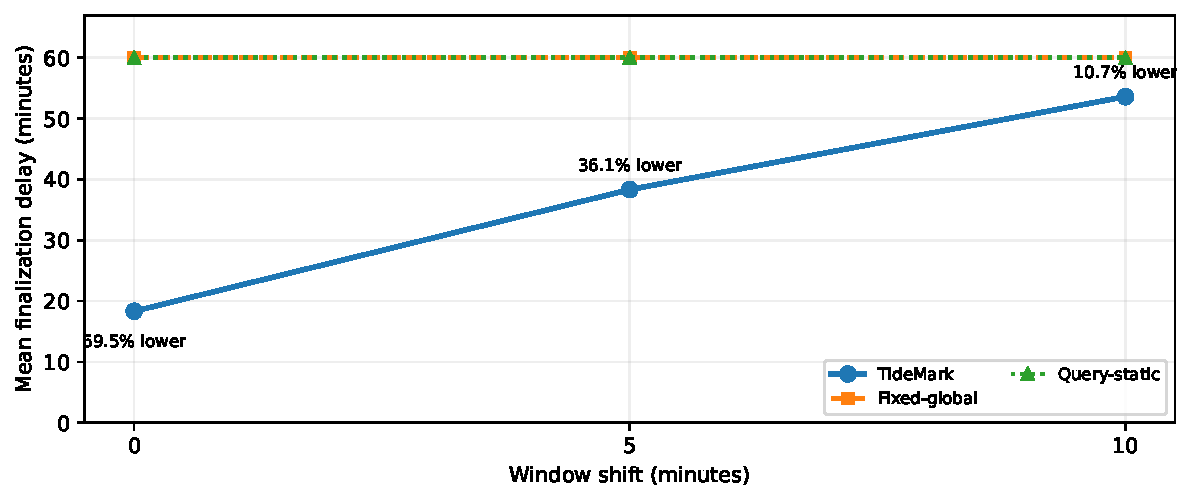
\includegraphics[width=\columnwidth]{fig8_phase_robustness.pdf}
  \caption{Window-phase sensitivity for 15-minute windows. Each offset
  changes the observed cell-window-query instances; the figure depicts
  independently calibrated policies rather than a paired comparison.}
  \label{fig:phase}
\end{figure}

The most revealing observation is the collapse of the \emph{latency advantage}, not a corresponding failure of empirical calibration. At the same nominal duration of 15 minutes, the mean delay rises from 18.33 minutes for aligned windows to 38.33 and 53.61 minutes at five- and ten-minute offsets (Fig.~\ref{fig:phase}). The gains against the 60-minute fixed-global rule consequently decline from 69.45\% to 36.12\% and 10.66\%. Yet the observed violation fractions are 0.2844\%, 0.2924\%, and 0.1246\%, all below the 1\% calibration budget. Thus, the method can remain empirically conservative while losing much of its opportunity to finalize early. This distinction matters: a policy can satisfy its risk target without providing useful latency reduction. The pattern is consistent with the audited 15-minute source-update cadence, but the separately generated test populations prevent a causal attribution to phase alone.

\begin{figure}[t]
  \centering
  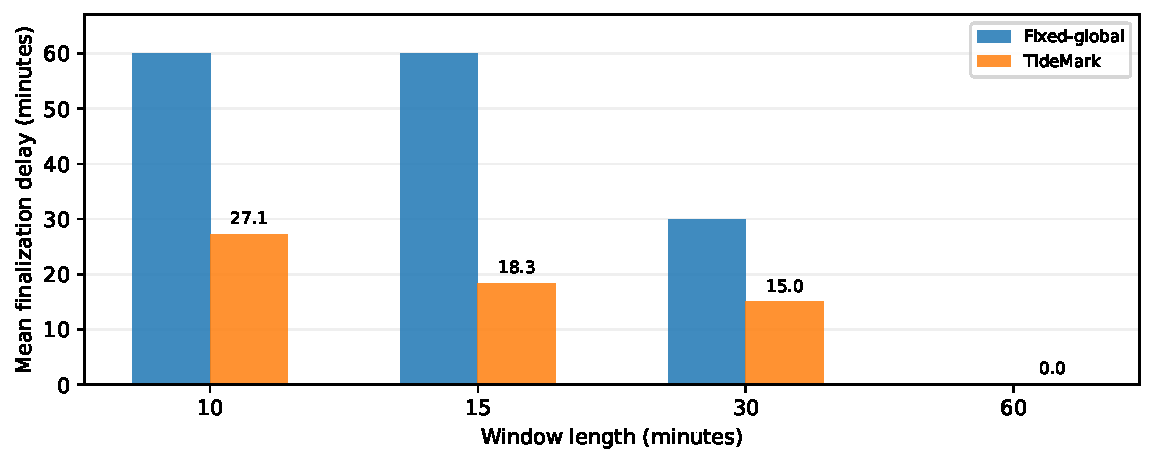
\includegraphics[width=\columnwidth]{fig9_window_duration.pdf}
  \caption{Window-duration sensitivity for aligned windows under the
  same query definitions and chronological protocol. At 60 minutes,
  the fixed-global and context-aware policies both select zero delay.}
  \label{fig:duration}
\end{figure}

Duration reveals a second limit (Fig.~\ref{fig:duration}). Relative to a \emph{recalibrated} fixed-global policy, TideMark saves 54.78\% for 10-minute windows (60.00 to 27.13 minutes) and 50.02\% for 30-minute windows (30.00 to 14.99 minutes). For aligned 60-minute windows, both policies select immediate finalization. Their zero additional delay does \emph{not} imply exact answers: the observed violation fraction is 0.3112\%. Rather, it means that the selected empirical tolerance can be met immediately even by a global rule, leaving no latency for contextual adaptation to recover. The six-way comparison therefore offers a more discriminating interpretation than a single headline improvement: the potential value of risk-calibrated finalization is determined jointly by query semantics, the candidate delay set, the availability process, and the chosen window geometry.

\subsection{RQ8: What is the offline processing cost?}
Table~\ref{tab:runtime} reports successful-stage runtimes for the full run on a Windows 11 workstation with an Intel64 Family 6 Model 154 CPU, 20 logical CPUs, DuckDB 1.5.5, an 8 GB DuckDB memory limit, and four configured threads (snapshot construction used two threads in the final resilient run). Typed ingestion dominates at 44.5 minutes, followed by evaluation at 16.3 minutes and snapshot construction at 12.3 minutes. The sum of successful-stage runtimes is about 76.2 minutes. Because earlier failed/restarted attempts are not included, this is not presented as end-to-end wall-clock time.

The ingest stage reads 154.86 GB in 2,671 s, corresponding to approximately 58 MB/s and 310k typed rows/s. These measurements show that the replay is practical on a single workstation, but they are not a distributed-system benchmark. The expensive replay is an offline calibration/evaluation procedure; in a prospective implementation, the policy decision would require a lookup over 279 rules for each $(\eps,\alpha)$ configuration. Neither live per-window overhead nor distributed-system throughput has been measured. The contribution evaluated here is finalization policy quality and its control semantics; end-to-end integration into a distributed engine remains future work.

\begin{table}[t]
\caption{Successful-stage full-run runtimes.}
\label{tab:runtime}
\centering
\begin{tabular}{lrr}
\toprule
Stage & Seconds & Minutes \\
\midrule
Ingest & 2671.24 & 44.52 \\
Audit & 182.69 & 3.04 \\
Snapshots & 738.90 & 12.32 \\
Evaluation & 980.68 & 16.34 \\
\midrule
Total & 4573.50 & 76.23 \\
\bottomrule
\end{tabular}
\end{table}

\section{Reproducibility and Artifact Trail}
The experiment is organized as a resumable, manifest-driven pipeline rather than as a monolithic notebook. The run manifest records the source file size (154,860,803,000 bytes), a hash of the first MiB, the parsed schema, Python/DuckDB/Pandas/NumPy versions, memory limit, and configured thread count. Each major stage writes a completion manifest and log; the evaluation manifest records the number of train, calibration, and test cell-window-query instances for every query. Heavy aggregation is executed in DuckDB, while Pandas receives only aggregated tables, reducing the risk that the evaluation logic silently depends on workstation memory.

The paper-facing artifact trail contains the exact configuration, split-day table, policy metrics, per-query metrics, day-level metrics, bootstrap intervals, delay-error curves, calibrated rules, and the post-hoc held-out stress-slice tables used to generate the robustness results. A separate timestamp-cadence audit and an independently recomputed held-out-day snapshot check are retained alongside the main run. The supplementary artifact now contains the complete six-configuration sensitivity return, with per-variant manifests, policy and per-query metrics, daily summaries, bootstrap intervals, delay curves, and calibration rules. The provided summary files were cross-checked against independent per-query, instance-weighted aggregations. Six variant folders report completed execution, although the archive includes only derived outputs rather than the raw AIS corpus. The raw AIS source cannot be reconstructed from these derived artifacts; the publicly distributable subset of the artifact can include code, manifests, derived summaries, and audits, subject to a data-licensing review. Full end-to-end reproduction still requires lawful access to the original AIS source and its recorded timestamps; the derived-output archive alone does not meet that requirement.

\section{Discussion and Limitations}
\subsection{Separating risk feasibility from latency opportunity}
The primary result has two parts that should not be conflated. First, a query-aware controller can meet the selected \emph{empirical} calibration target on held-out windows without imposing one global delay on all answers. In the aligned 15-minute experiment, its average delay is 18.33 minutes, compared with 60.00 minutes for the recalibrated global rule, and its observed violation fraction is 0.2844\%. Second, satisfying the risk criterion does not itself imply meaningful latency savings. The ten-minute phase shift retains a low violation fraction but produces only a 10.66\% gain; with aligned 60-minute windows there is no gain because the global rule also chooses zero delay. These outcomes expose the two quantities a practitioner must measure separately: \emph{risk feasibility} and \emph{latency opportunity}.

The result also helps locate the scientific contribution. It is not a claim that the system predicts every late record, nor that contextual calibration universally dominates a fixed waiting policy. The contribution is the explicit recognition that the \emph{decision object} is the answer and that the payoff of this decision is empirically conditioned by window semantics and source cadence. In this respect, an apparently adverse sensitivity result is methodologically valuable: it prevents a favorable, aligned configuration from being mistaken for an architecture-independent improvement.

\subsection{Scope of inference}
Five restrictions are material. (i) The risk budget $\alpha$ is enforced on the calibration sample, without a distribution-free guarantee on future windows, individual days, or shifted regimes. (ii) The reconstructed \texttt{ProcessedDate} is a source/database availability proxy. Its 15-minute cadence must not be translated into physical AIS transmission or network-reception latency. (iii) The analysis concerns count-like aggregates over eligible, nonempty spatial windows with positive closed-corpus values. Empty windows and richer operators---joins, quantiles, top-$k$ results, sketches, or learned outputs---would require adapted loss functions and independent evaluation. (iv) Fixed-global and query-static policies are controlled calibration baselines; the study does not provide a head-to-head implementation comparison with modern adaptive or keyed watermarks in a live engine. (v) Window configurations differ in their eligible cell-window-query populations and are separately recalibrated. The reported phase and duration contrasts are therefore descriptive, not paired causal estimates.

In addition, the closed-corpus reference answer includes all eligible historical records, even those arriving after the largest candidate delay. Rare residual violations can therefore persist even for the offline oracle, whose future knowledge is unavailable in deployment. We have not measured the end-to-end throughput or memory impact of embedding the controller as a native Flink or Beam trigger; the low-cost lookup-table design is an implementation argument rather than a measured distributed-systems result.

\subsection{Deployment implication: two control planes}
The practical consequence is an architectural separation. The stream engine continues to govern record progress, provisional updates, and safe state reclamation through its ordinary event-time mechanisms. A second, answer-oriented controller uses the observable context at window close to schedule a \emph{user-visible final} result. Records arriving before that decision revise provisional state; subsequent records require an explicit application policy, such as correction, retraction, or an accepted approximation. Declaring output final does not authorize early state eviction.

Since the controller's evidence is historical, a production design must also monitor calibration drift. A rise in observed post-final discrepancies should trigger rule recalibration, conservative hierarchical fallback, or a temporary return to ordinary watermark-driven finalization. This suggests a larger research direction: stream systems in which input progress, answer quality, and confidence in the quality estimate are represented separately. The present experiments motivate that direction but do not implement its full online monitoring layer.

\section{Conclusion}
Stream finality has traditionally been discussed in the language of arriving records. The evidence presented here supports a complementary language: \emph{how much uncertainty remains in the answer that will be exposed to a consumer?} We formalized this question through \stablecq{} and instantiated it with the transparent, hierarchically calibrated \tidemark{} policy. On 44.3 million held-out cell-window-query instances from an 828.9-million-record historical replay, the aligned 15-minute setting shows a 69.45\% reduction in mean finalization delay with 0.2844\% observed violations under a 1\% empirical calibration budget. Six completed window configurations then delimit that achievement: gains diminish under phase shifts, and disappear when a global rule already supports immediate finalization. The essential lesson is not that one rule is optimal for every stream. It is that progress of the input and stability of a query answer are distinct system decisions; recognizing their separation makes both the benefit and the limits of early finalization measurable.


\section*{Acknowledgment}
This work was supported by grant FD-20/IT-3/002.

\section*{AI-Generated Content Acknowledgement}
OpenAI ChatGPT (GPT-5.6 and GPT-6) was used to assist with English-language editing, organization and literature positioning; with LaTeX and plotting code; and with checks and secondary summaries of author-provided experimental outputs. These contributions affect the Abstract, Introduction, Related Work, Discussion, Conclusion, result presentation, and supplementary verification scripts. The primary historical replay and evaluation outputs were generated using the authors' pipeline. The authors are responsible for validating all generated content, analyses, source code, figures, and bibliographic records before submission.

\balance
\begin{thebibliography}{99}

\bibitem{babcock2002streams}
B. Babcock, S. Babu, M. Datar, R. Motwani, and J. Widom,
``Models and issues in data stream systems,'' in \emph{Proc. ACM PODS}, 2002, pp. 1--16, doi: 10.1145/543613.543615.

\bibitem{abadi2003aurora}
D. J. Abadi, D. Carney, U. Cetintemel, M. Cherniack, C. Convey, S. Lee, M. Stonebraker, N. Tatbul, and S. Zdonik,
``Aurora: A new model and architecture for data stream management,'' \emph{VLDB Journal}, vol. 12, no. 2, pp. 120--139, 2003, doi: 10.1007/s00778-003-0095-z.

\bibitem{golab2003issues}
L. Golab and M. T. {\"O}zsu, ``Issues in data stream management,'' \emph{ACM SIGMOD Rec.}, vol. 32, no. 2, pp. 5--14, 2003, doi: 10.1145/776985.776986.

\bibitem{abadi2005borealis}
D. J. Abadi \emph{et al.}, ``The design of the Borealis stream processing engine,'' in \emph{Proc. CIDR}, 2005, pp. 277--289.

\bibitem{arasu2006cql}
A. Arasu, S. Babu, and J. Widom, ``The CQL continuous query language: Semantic foundations and query execution,'' \emph{VLDB J.}, vol. 15, no. 2, pp. 121--142, 2006, doi: 10.1007/s00778-004-0147-z.

\bibitem{akidau2015dataflow}
T. Akidau, R. Bradshaw, C. Chambers, S. Chernyak, R. J. Fern\'andez-Moctezuma, R. Lax, S. McVeety, D. Mills, F. Perry, E. Schmidt, and S. Whittle,
``The Dataflow Model: A practical approach to balancing correctness, latency, and cost in massive-scale, unbounded, out-of-order data processing,'' \emph{Proc. VLDB Endow.}, vol. 8, no. 12, pp. 1792--1803, 2015, doi: 10.14778/2824032.2824076.

\bibitem{fragkoulis2024survey}
M. Fragkoulis, P. Carbone, V. Kalavri, and A. Katsifodimos,
``A survey on the evolution of stream processing systems,'' \emph{VLDB Journal}, vol. 33, no. 2, pp. 507--541, 2024, doi: 10.1007/s00778-023-00819-8.

\bibitem{awad2019adaptive}
A. Awad, J. Traub, and S. Sakr,
``Adaptive watermarks: A concept drift-based approach for predicting event-time progress in data streams,'' in \emph{Proc. EDBT}, 2019, pp. 622--625, doi: 10.5441/002/EDBT.2019.71.

\bibitem{yasser2025keyed}
T. Yasser, T. Arafa, M. ElHelw, and A. Awad,
``Keyed watermarks: A fine-grained watermark generation for Apache Flink,'' \emph{Future Generation Computer Systems}, vol. 169, Art. no. 107796, 2025, doi: 10.1016/j.future.2025.107796.

\bibitem{stonebraker2005requirements}
M. Stonebraker, U. {\c{C}}etintemel, and S. B. Zdonik, ``The 8 requirements of real-time stream processing,'' \emph{ACM SIGMOD Rec.}, vol. 34, no. 4, pp. 42--47, 2005, doi: 10.1145/1107499.1107504.

\bibitem{zaharia2013dstreams}
M. Zaharia, T. Das, H. Li, T. Hunter, S. Shenker, and I. Stoica,
``Discretized streams: Fault-tolerant streaming computation at scale,'' in \emph{Proc. ACM SOSP}, 2013, pp. 423--438, doi: 10.1145/2517349.2522737.

\bibitem{murray2013naiad}
D. G. Murray, F. McSherry, R. Isaacs, M. Isard, P. Barham, and M. Abadi,
``Naiad: A timely dataflow system,'' in \emph{Proc. ACM SOSP}, 2013, pp. 439--455, doi: 10.1145/2517349.2522738.

\bibitem{chandramouli2014trill}
B. Chandramouli, J. Goldstein, M. Barnett, R. DeLine, D. Fisher, J. C. Platt, J. F. Terwilliger, and J. Wernsing,
``Trill: A high-performance incremental query processor for diverse analytics,'' \emph{Proc. VLDB Endow.}, vol. 8, no. 4, pp. 401--412, 2014, doi: 10.14778/2735496.2735503.

\bibitem{carbone2017flinkstate}
P. Carbone, S. Ewen, G. F\'ora, S. Haridi, S. Richter, and K. Tzoumas,
``State management in Apache Flink: Consistent stateful distributed stream processing,'' \emph{Proc. VLDB Endow.}, vol. 10, no. 12, pp. 1718--1729, 2017, doi: 10.14778/3137765.3137777.

\bibitem{akidau2013millwheel}
T. Akidau \emph{et al.}, ``MillWheel: Fault-tolerant stream processing at internet scale,'' \emph{Proc. VLDB Endow.}, vol. 6, no. 11, pp. 1033--1044, 2013, doi: 10.14778/2536222.2536229.

\bibitem{carbone2015flink}
P. Carbone, A. Katsifodimos, S. Ewen, V. Markl, S. Haridi, and K. Tzoumas, ``Apache Flink: Stream and batch processing in a single engine,'' \emph{IEEE Data Eng. Bull.}, vol. 38, no. 4, pp. 28--38, 2015.

\bibitem{armbrust2018structured}
M. Armbrust \emph{et al.}, ``Structured Streaming: A declarative API for real-time applications in Apache Spark,'' in \emph{Proc. ACM SIGMOD}, 2018, pp. 601--613, doi: 10.1145/3183713.3190664.

\bibitem{li2008ooo}
J. Li, K. Tufte, V. Shkapenyuk, V. Papadimos, T. Johnson, and D. Maier,
``Out-of-order processing: A new architecture for high-performance stream systems,'' \emph{Proc. VLDB Endow.}, vol. 1, no. 1, pp. 274--288, 2008, doi: 10.14778/1453856.1453890.

\bibitem{chandramouli2018impatience}
B. Chandramouli, J. Goldstein, and Y. Li,
``Impatience is a virtue: Revisiting disorder in high-performance log analytics,'' in \emph{Proc. IEEE ICDE}, 2018, pp. 677--688, doi: 10.1109/ICDE.2018.00067.

\bibitem{traub2018scotty}
J. Traub \emph{et al.}, ``Scotty: Efficient window aggregation for out-of-order stream processing,'' in \emph{Proc. IEEE ICDE}, 2018, pp. 1304--1307, doi: 10.1109/ICDE.2018.00135.

\bibitem{traub2021scotty}
J. Traub \emph{et al.}, ``Scotty: General and efficient open-source window aggregation for stream processing systems,'' \emph{ACM Trans. Database Syst.}, vol. 46, no. 1, Art. no. 1, 2021, doi: 10.1145/3433675.

\bibitem{wu2006cep}
E. Wu, Y. Diao, and S. Rizvi, ``High-performance complex event processing over streams,'' in \emph{Proc. ACM SIGMOD}, 2006, pp. 407--418, doi: 10.1145/1142473.1142520.

\bibitem{cugola2012cep}
G. Cugola and A. Margara, ``Processing flows of information: From data stream to complex event processing,'' \emph{ACM Comput. Surv.}, vol. 44, no. 3, Art. no. 15, 2012, doi: 10.1145/2187671.2187677.

\bibitem{meehan2015sstore}
J. Meehan \emph{et al.}, ``S-Store: Streaming meets transaction processing,'' \emph{Proc. VLDB Endow.}, vol. 8, no. 13, pp. 2134--2145, 2015, doi: 10.14778/2831360.2831367.

\bibitem{hellerstein1997online}
J. M. Hellerstein, P. J. Haas, and H. J. Wang, ``Online aggregation,'' in \emph{Proc. ACM SIGMOD}, 1997, pp. 171--182, doi: 10.1145/253260.253291.

\bibitem{kiersztyn2024aisintegrity}
A. Kiersztyn, D. Czerwi{\'n}ski, E. Czerma{\'n}ski, A. Oniszczuk-Jastrz{\k{a}}bek, K. Smoli{\'n}ski, P. Miazek, T. Laskowicz, J. Jankiewicz, A. Rzepka, and R. Mi{\'s}kiewicz,
``Data integrity analysis on the example of AIS database,'' \emph{Scientific Papers of Silesian University of Technology: Organization and Management Series}, no. 208, pp. 155--170, 2024, doi: 10.29119/1641-3466.2024.208.9.

\bibitem{kiersztyn2025aisaccuracy}
A. Kiersztyn, D. Czerwinski, A. Oniszczuk-Jastrzabek, E. Czermanski, and A. Rzepka,
``Data integrity versus inference accuracy in large AIS datasets,'' in \emph{Sustainable Data Management: Navigating Big Data, Communication Technology, and Business Digital Leadership}, vol. 2, R. K. Hamdan, Ed. Springer, 2025, pp. 405--414, doi: 10.1007/978-3-031-83915-3\_32.

\bibitem{czerwinski2023offshore}
D. Czerwi{\'n}ski, A. Kiersztyn, S. Przy{\l}ucki, A. Oniszczuk-Jastrz{\k{a}}bek, and E. Czerma{\'n}ski,
``Analysis of passenger ships activity in the oil and gas offshore shipping sector in the North Sea,'' \emph{Scientific Journals of the Maritime University of Szczecin}, vol. 75, no. 147, pp. 68--78, 2023, doi: 10.17402/575.

\bibitem{kiersztyn2025vesselstatus}
A. Kiersztyn, D. Czerwinski, K. Kiersztyn, E. Czermanski, and A. Oniszczuk-Jastrzabek,
``Predicting vessel movement status using temporal-spatial AIS data and machine learning,'' in \emph{Proc. IEEE Int. Conf. Data Mining Workshops (ICDMW)}, 2025, pp. 1776--1784, doi: 10.1109/ICDMW69685.2025.00213.

\end{thebibliography}
\end{document}
